\documentclass[12pt,english]{article}
\usepackage[cm]{fullpage}
\usepackage[utf8]{inputenc}
\usepackage[T1]{fontenc}
\usepackage{lmodern}
\usepackage[main=english]{babel}
\usepackage{mathtools}
\usepackage{siunitx}
\usepackage[dvipsnames]{xcolor}
\usepackage{listings}
\lstset{
	language=Python,
	morekeywords={as,assert,with},
	basicstyle=\footnotesize\ttfamily,
	keywordstyle=\bfseries\color{Plum},
	identifierstyle=\color{Red},
	stringstyle=\color{Green},
	commentstyle=\color{Gray},
	showstringspaces=false,
	tabsize=4,
	breaklines=true,
	prebreak=\mbox{\(\hookleftarrow\)},
	numbers=left,
	numberstyle=\footnotesize\color{darkgray},
	frame=leftline
}
\usepackage{tikz}
\usepackage[labelfont={bf},labelsep=endash]{caption}
\usepackage{hyperref}
\hypersetup{
	colorlinks=true,
	linkcolor=blue,
	urlcolor=cyan
}

\makeatletter
	\renewcommand*\and{\newline}
	\let\old@itemize\itemize%
	\renewcommand\itemize{
		\parskip=0pt
		\old@itemize%
	}
	\let\old@enditemize\enditemize%
	\renewcommand\enditemize{
		\old@enditemize%
		\parskip=\baselineskip%
	}
	\let\old@enumerate\enumerate%
	\renewcommand\enumerate{
		\parskip=0pt
		\old@enumerate%
	}
	\let\old@endenumerate\endenumerate%
	\renewcommand\endenumerate{
		\old@endenumerate%
		\parskip=\baselineskip%
	}
	\renewcommand*\@maketitle{
		\begin{titlepage}
			\begin{flushright}
				ISEP
			\end{flushright}
			\begin{center}
				\vfill
				{\Huge\@title}

				\vspace{5cm}
				{\Large\@author}

				\vfill
				{\large\@date}
			\end{center}
		\end{titlepage}
	}
	\let\old@appendix\appendix
	\renewcommand*\appendix{
		\newpage
		\part*{Appendix}\addcontentsline{toc}{part}{Appendix}
		\old@appendix%
	}
	\addto\captionsenglish{
		\renewcommand\contentsname{Table of Contents}
	}
\makeatother

\author{
	Cyprien \textsc{Bariant} %TODO
	\and
	Tanguy \textsc{Berthoud} 60989
	\and
	Thibault \textsc{du Buisson de Courson} %TODO
}
\title{
	\textbf{PROJECT}\\
	Advanced Algorithmic and Programming
}
\begin{document}
	\maketitle\newpage
	\thispagestyle{empty}
	\tableofcontents
	\listoffigures
	\listoftables
	\newpage
	\parskip=\baselineskip%

	\section{Creating a graph from GTFS data}\label{sec:step:1}
	\subsection{Importing relevant GTFS data}\label{sec:step:1.1}

	Our city of choice for the project is Phoenix, in Arizona.\\
	We use the public data available here: \url{https://transitfeeds.com/p/valley-metro/68/latest}

	The difficulty here was to import the relevant data and convert it to a graph.
	Some Python libraries seem to exist but none was convenient for the project, so we needed to transform the data manually.\\
	After reading documentation on GTFS, we needed only two files from the data feed: \texttt{stops.txt} and \texttt{stop\_times.txt}.

	\begin{center}
		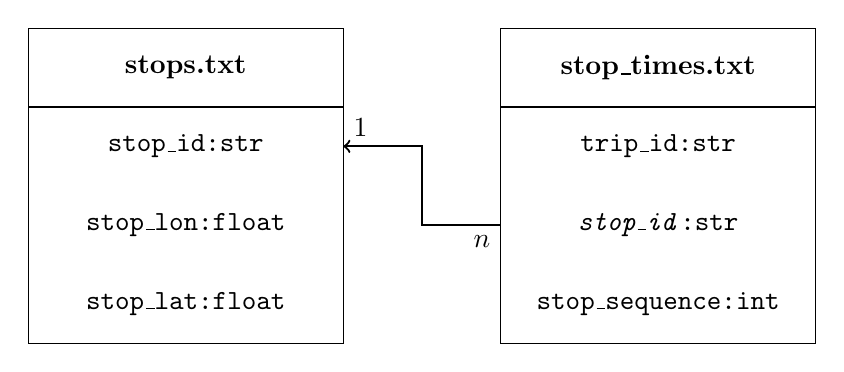
\begin{tikzpicture}
			\draw (0,3) rectangle +(4,1);
			\node at (2,3.5) {\bfseries stops.txt};
			\draw (0,0) rectangle +(4,4);
			\node at (2,2.5) {\ttfamily\bfseries stop\_id:str};
			\node at (2,1.5) {\ttfamily stop\_lon:float};
			\node at (2,.5) {\ttfamily stop\_lat:float};

			\draw (6,3) rectangle +(4,1);
			\node at (8,3.5) {\bfseries stop\_times.txt};
			\draw (6,0) rectangle +(4,4);
			\node at (8,2.5) {\ttfamily\bfseries trip\_id:str};
			\node at (8,1.5) {\ttfamily \textit{stop\_id}:str};
			\node at (8,.5) {\ttfamily stop\_sequence:int};

			\draw[thick,->] (6,1.5) node[anchor=north east] {\(n\)} -- ++(-1,0) -- ++(0,1) -- +(-1,0) node[anchor=south west] {\(1\)};
		\end{tikzpicture}
		\captionof{figure}{Database representation of the relevant GTFS files}
	\end{center}

	The nodes of the graph are directly given by the file \texttt{stops.txt}, so we can just parse the file to import them.
	This is done in the \texttt{import\_nodes} function of \hyperref[sec:code:gtfs]{\ttfamily gtfs.py}.

	Whereas the edges need some operations:
	\begin{enumerate}
		\item Parse the file
		\item Regroup in order the stops in the same trips
		\item Create edges between consecutive stops in a trip
	\end{enumerate}
	This is done in the \texttt{import\_edges} function of \hyperref[sec:code:gtfs]{\ttfamily gtfs.py}.

	\subsection{Creating a graph}\label{sec:step:1.2}

	The \texttt{Graph} class is in \hyperref[sec:code:graph]{\ttfamily graph.py}.

	The class supports weighted directed graphs, but unweighted or undirected graphs can also be created.\\
	The class constructor accepts an optional parameter which is a callback to compute weight from two given nodes.
	In our case, this function takes two \texttt{Stop} (defined in \hyperref[sec:code:gtfs]{\ttfamily gtfs.py}) instances and returns the Euclidian distance between them: \[
		\text{compute\_weight}: (s,s') \mapsto \sqrt{\left(s'_\text{lat} - s_\text{lat}\right)^2 + \left(s'_\text{lon} - s_\text{lon}\right)^2}
	\]
	If this parameter is not passed, all edge weights will be set to \(0\).\\
	The support for directions comes from the \texttt{neighbors\_in} and \texttt{neighbors\_out} methods.
	The method \texttt{neighbors} can be used instead for undirected graphs.

	After testing the pathfinding methods (see \autoref{sec:step:2}), we realized that our way of storing neighbors was not optimized.\\
	Indeed we stored the neighbors in a huge adjacency list.
	So when we needed to compute some neighbors, we had to search in the whole list for neighbors.\\
	So we optimized this aspect.
	We are now storing the neighbors of a node inside the \texttt{Node} object itself.
	This implementation has redundancy in memory, but fetching the neighbors of a node is now \(\mathcal{O}(1)\) for the \texttt{neighbors\_out} and \texttt{neighbors\_in} methods, but not for \texttt{neighbors} since it computes the union of two sets.

	\subsection{Results}\label{sec:results:1}

	\begin{itemize}
		\item \(7982\) lines from \texttt{stops.txt} were imported to \(7982\) nodes in the graph.
		\item \(1720661\) lines from \texttt{stop\_times.txt} were imported to \(8462\) edges in the graph.\\
		This is not surprising, because one line is used for a single stop in a single trip at certain hours: there are a lot of redundancies.
	\end{itemize}

	\begin{center}
		\begin{tabular}{r c c c}
			& \textbf{\ttfamily import\_stops} & \textbf{\ttfamily import\_edges} & \textbf{\ttfamily Graph}\\
			\hline\hline
			Before neighbors optimization & \num{38.61} & \num{4211.02} & \num{78.64}\\
			& \num{31.75} & \num{5036.29} & \num{49.05}\\
			& \num{44.50} & \num{5085.64} & \num{68.83}\\
			& \num{28.56} & \num{3786.03} & \num{43.43}\\
			& \num{26.48} & \num{4070.86} & \num{43.62}\\
			\hline
			After neighbors optimization & \num{27.24} & \num{4931.54} & \num{155.09}\\
			& \num{29.34} & \num{3610.81} & \num{74.15}\\
			& \num{49.93} & \num{4096.88} & \num{115.51}\\
			& \num{28.70} & \num{3279.42} & \num{86.15}\\
			& \num{26.39} & \num{3685.92} & \num{82.94}\\
		\end{tabular}
		\captionof{table}{Execution time (\si{\milli\second}) for the graph creation over several tries}
		\label{tab:exectime:graph}
	\end{center}
	We see in this \autoref{tab:exectime:graph} that after the optimization described in \autoref{sec:step:1.2}, the execution time for the \texttt{Graph} instanciation has increased from an average of \SI{56.71}{\milli\second} to \SI{102.77}{\milli\second}.
	This can be explained by the new storage method of neighbors: we need to add two different tuples into two different sets.

	%TODO visual graph ?

	\section{Finding the shortest paths}\label{sec:step:2}

	%TODO

	\appendix
	\section{\texttt{gtfs.py}}\label{sec:code:gtfs}
	\lstinputlisting{src/gtfs.py}

	\section{\texttt{graph.py}}\label{sec:code:graph}
	\lstinputlisting{src/graph.py}

	\section{\texttt{pathfinding.py}}\label{sec:code:pathfinding}
	\lstinputlisting{src/pathfinding.py}
\end{document}
